\chapter{Gauß-Layout-System}\label{chap:gausspage}

Dieses Kapitel beschreibt das allgemeine Layoutsystem zur Erstellung von
Inhalten und Hintergründen im Gaußraster des Corporate Designs.
Es findet als Basis unter anderem bei der Darstellung von Titelseiten oder
Veranstaltungspostern Anwendung. Die hier beschriebenen Befehle und Optionen
können daher in weiten Teilen auf alle Konstruke in \tubslatex angewendet
werden, die im Gauß-Layout dargestellt werden.

Es gibt grundlegend drei verschiedene Möglichkeiten das Gauß-Layout-System
zu nutzen:
\begin{itemize}
  \item Definition einer Hintergrunddarstellung,
  \item Verwendung von Textboxen,
  \item Kombination von Hintergrundelementen und Textboxen,
\end{itemize}
wobei die Letztgenannte den Regelfall darstellt.

\section{Hintergrund-Layout}

\begin{Declaration}
  \Macro{bglayout}\OParameter{Optionen}\Parameter{Layout}
\end{Declaration}

Mit Hilfe des Befehls \Macro{bglayout} kann das Hintergrundlayout im Gaußraster gesetzt werden.
% Dies hat in etwa dieselbe Funktionalität wie vorbedrucktes Papier.
Alle Komponenten werden im Hintergrund und unabhängig vom Inhalt der Seite
dargesetellt.

Folgende \PName{Optionen} können gewählt werden:

\begin{Declaration}
  \KOption{sender}\PName{top/bottom}
\end{Declaration}

Steuert die Positionierung des Absenderbereiches.
Der Wert \PValue{top} platziert den Absenderbereich am oberen,
der Wert \PValue{bottom} am unteren Ende des Blattes.

\begin{Declaration}
  \KOption{pages}\PName{all/single}
\end{Declaration}

Legt fest für welche Seiten die aktuelle Einstellung gelten soll.
Der Wert \PValue{all} besagt, dass es für alle folgenden Seiten gelten soll,
während mit \PValue{single} die Darstellung nur auf der aktuellen Seite geändert 
wird.

\subsection{Elemente}

\begin{Declaration}
  \Macro{bgelement}\OParameter{Darstellung}\PParameter{Höhe}
\end{Declaration}

Erstellt ein Hintergrundelement im Gaußraster mit angegebener \PName{Höhe}.
Diese gibt an wieviele Segmente des Gauß-Layouts für das aktuelle Element
verwendet werden sollen.
Die Segmente werden debei von oben nach unten Belegt.
Abhängig von der Position des Absenderbereiches werden die Segmente
entweder nach unten kleiner (Absender oben) oder größer (Absender unten).

\noindent\begin{minipage}{0.4\textwidth}
Pro Seite stehen allgemein maximal 8 (Hochformat) bzw. 6 (Querformat)
Segmente zur Verfügung. Werden mehr belegt, so kommt es zu einer Fehlermeldung.
\end{minipage}
\begin{minipage}{0.6\textwidth}\centering
\begin{minipage}[b]{0.4\textwidth}\centering
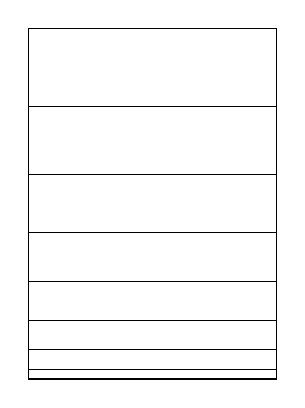
\begin{tikzpicture}[scale=1.5]
  \def\tikzpageheight{2.97}
  \def\tikzpagewidth{2.1}
  \draw (0,0) rectangle (\tikzpagewidth, \tikzpageheight);
  \foreach \i in {1,3,6,10,15,21,28}{%
    \draw (0, \i*\tikzpageheight/36) -- (\tikzpagewidth, \i*\tikzpageheight/36);
  }
\end{tikzpicture}\\
Hochformat\\ (8 Segmente)
\end{minipage}
\begin{minipage}[b]{0.45\textwidth}\centering
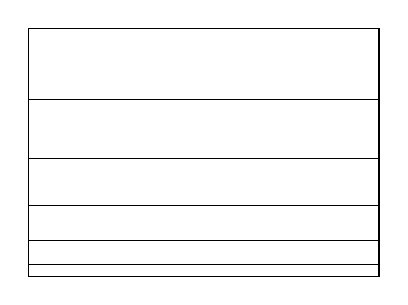
\begin{tikzpicture}[scale=1.5]
  \def\tikzpageheight{2.1}
  \def\tikzpagewidth{2.97}
  \draw (0,0) rectangle (\tikzpagewidth, \tikzpageheight);
  \foreach \i in {1,3,6,10,15}{%
    \draw (0, \i*\tikzpageheight/21) -- (\tikzpagewidth, \i*\tikzpageheight/21);
  }
\end{tikzpicture}\\
Querformat\\ (6 Segmente)
\end{minipage}
\end{minipage}
\vspace*{0pt}


Der optionale Parameter \PName{Darstellung} kann die folgenden Einstellungen verarbeiten:


\begin{Declaration}
  \KOption{bgcolor}\PName{Farbe}\\
  \KOption{bgimage}\PName{Bild-Datei}\\
  \KOption{imagefit}\PName{Darstellungsoption}
\end{Declaration}

Mit \OptionValue{bgcolor}{Farbe} wird das Hintergrundelement mit der angegebenen
Farbe gefüllt.

Die Option \OptionValue{bgimage}{Bild-Datei} erlaubt dagegen die Darstellung
eines Hintergrundbildes im Element.
Da der Darstellungsbereich fest vorgegeben ist, muss das eingebundene Bild
in diesen Bereich eingepasst werden. Dies geschieht automatisch, die Art
der Einpassung lässt sich aber mit der Option \Option{imagefit} kontrollieren.
Sie erlaubt folgende Einstellungen:


\begin{desctable}
\entry{\PValue{clipped}}{%
  Automatisches Abschneiden. Dies ist die Standardeinstellung.
}
\entry{\PValue{clipx}/\PValue{fitheight}}{%
  Abschnitt horizontal.
}
\entry{\PValue{clipy}/\PValue{fitwidth}}{%
  Abschnitt vertikal.
}
\entry{\PValue{scaled}}{%
  Horizontale \emph{und} vertikale Skalierung.
}
\end{desctable}


\begin{Declaration}
  \Macro{showtubslogo}\OParameter{Position}
\end{Declaration}

Bewirkt Darstellung des TU-Siegelbandlogos im aktiven Layout.
Die Option \PName{Position} erlaubt die Angabe der Darstellungsseite
(links/rechts). Standardmäßig wird das Logo links bzw. innen dargestellt.

\begin{Declaration}
  \Macro{showlogo}\PParameter{Logo}
\end{Declaration}

Bewirkt Darstellung eines Individuellen Logos im aktuellen Layout.
\PName{Logo} kann dabei entweder einfacher Text oder auch ein 
mit \Macro{includegraphics} eingebundenes Bild sein.
In diesem Fall wird eine Eingebundene Grafik automatisch auf die korrekte
Höhe skaliert (solange in den Optionen nicht anders angegeben).

Die Positionierung wird automatisch an die Position des Absenderbereichs und
die Positionierung des Siegelbandlogos angepasst.
Wird dies links bzw. innen platziert, so steht das individuelle
Logo rechts bzw. außen.

\begin{Declaration}
  \Macro{showtopline}
\end{Declaration}

Bewirkt Darstellung einer Trennlinie zwischen Absender und Kommunikationsbereich
im aktuellen Layout.



\begin{lstlisting}
\bglayout[pages=single]{%
  \showtubslogo
  \bgelement{2}
  \bgelement{3}
  \bgelement{3}
}
\end{lstlisting}


\section{Text-Boxen}

\begin{Declaration}
  \XMacro{begin}\PParameter{\Environment{gaussbox}}%
          \OParameter{Optionen}%
          \OParameter{hPos}%
          \Parameter{vPos}%
          \Parameter{Breite}%
          \Parameter{Höhe}\\
  \quad\dots\\
  \XMacro{end}\PParameter{gaussbox}
\end{Declaration}


\section{Kombination}

\begin{Declaration}
  \XMacro{begin}\PParameter{\Environment{gausspage}}%
    \OParameter{Optionen}\\
  \quad\dots\\
  \XMacro{end}\PParameter{gausspage}
\end{Declaration}


\begin{figure}\centering
  \fboxsep0mm
  \begin{minipage}{0.35\textwidth}
    \fbox{\includegraphics[width=\textwidth,page=1]{examples/gausssegments.pdf}}
    \subcaption{Absenderbereicht oben}\label{fig:gausspage:topsender}
  \end{minipage}
  \quad
  \begin{minipage}{0.35\textwidth}
    \fbox{\includegraphics[width=\textwidth,page=2]{examples/gausssegments.pdf}}
    \subcaption{Absenderbereicht unten}\label{fig:gausspage:bottomsender}
  \end{minipage}
  \caption{Gaußraster mit möglichen Logo-Positionen}\label{fig:gausspage}
\end{figure}




\begin{Declaration}
  \Macro{showdesignhelper}
\end{Declaration}

